\begin{homeworkProblem}[Quiz Problem 2, Week 1]
Okay, after reading question 2 on the quiz, it seems that it is ambiguously phrased. To that end, there are two equally acceptable ways in which to read the problem. It was also the case that students chose to write both the distance from the negative charge instead of the positive charge. For this reason, I had any number of 4 different solutions available to me when I was grading your quizzes. Needless to say, this made determining if you obtained the right answer very annoying. It's not your fault; it's just how life goes sometimes.


What I would like to do is walk you through each of the versions of the problem that you guys tried to solve and to show you all the ways in which you could have been right. This way, if you see that I deducted too many points from your quiz and you think that you deserve more credit, then you can come talk to me on reasonable grounds. I start by introducing the original/provided problem statement in bold. After this, I will solve a version of this problem statement according to how it \textbf{could have been read}.


Below follow two sections: 1a and 1b. 1a and 1b are related in that the problem to solve is similar. The only difference is which charge is selected to have the larger magnitude, the negative charge or the positive charge. In each section, I will supply the \textbf{version of the problem statement that could have been used to generate the associated problem}.

\begin{homeworkSection}{Problem 1a}
Supplied problem statement: \textbf{You are given two point charges, one positive and one negative, separated by distance  ``d''. The positive charge has 6 times the amount of charge on the negative charge. Where would you place a third charge so that the net electrostatic force on it is zero. Give answer in terms of ``d'' as measured from the positive charge.}


Interpreted problem statement: \textbf{You are given two point charges, one positive and one negative. These two charges are separated by distance ``d''. The positive charge is} 6 times larger than the negative charge. \textbf{Where would you place a third charge so that the net electrostatic force on it is zero. Give answer in terms of ``d'' as measured from the positive charge.}

\begin{figure}%
\centering
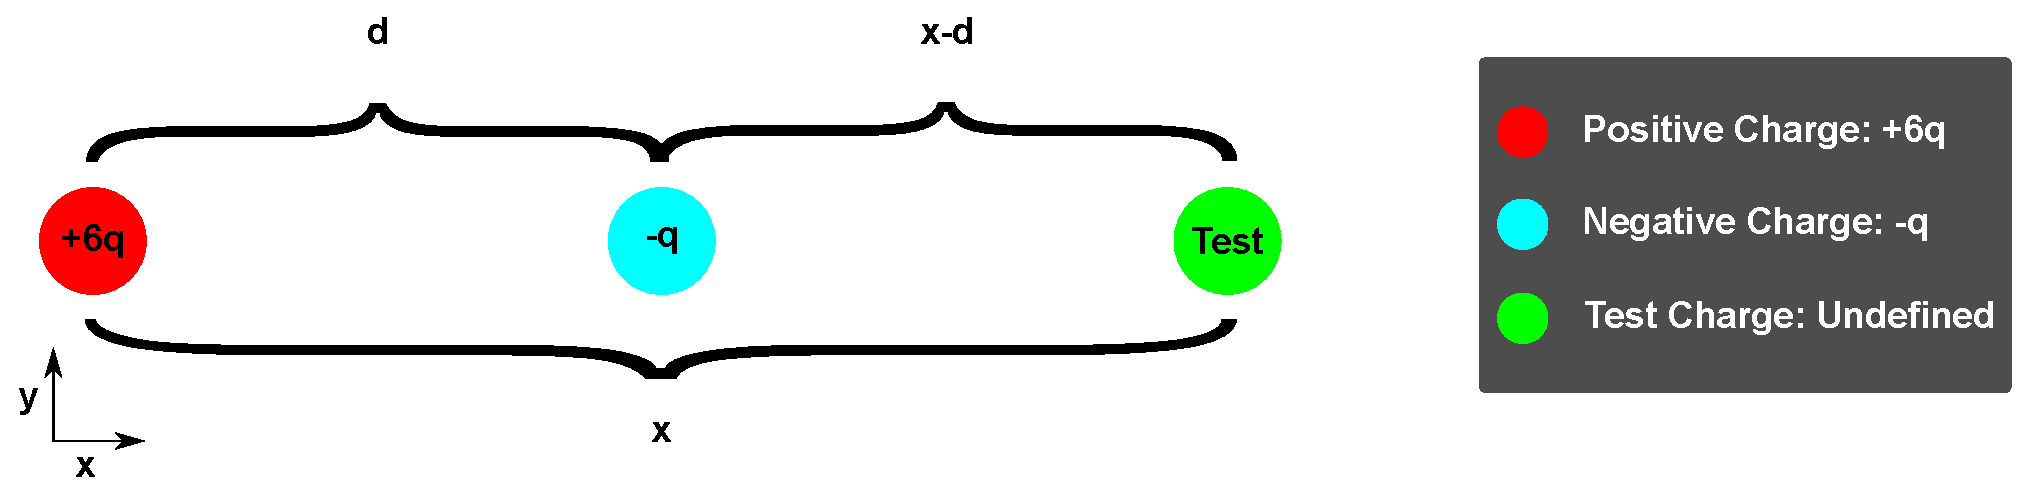
\includegraphics[width=\columnwidth]{1a.eps}%

\caption{Schematic for problem 1a. The key that describes the charges is redundant}%
\label{fig:1a}%
\end{figure}

The problem asks us to solve where $\vec{F}_{\text{test\,charge}} = 0 = q_{\text{test\,charge}}*\vec{E}_{\text{wherever\,the\,test\,charge\,is}}$. It is easy to realize in that equation that it does not matter what the test charge is. No matter if it's positive or negative or if the magnitude of that charge is very large or very small, $\vec{F}_{\text{test\,charge}}=0$ whenever $\vec{E}_{\text{wherever\,the\,test\,charge\,is}} = 0$. 


Let's consider all the places where the electric field and, hence, the force on the test charge, can be zero. First, it must be realized that the $\vec{E}$ field can only be zero on the line connecting our charges. If you consider the electric field at points off of the line connecting the charges you will find that the y-components of the electric-field can never cancel. However, on the line connecting the charges there is no y-component of the electric field, at all, for either charge. Thus, the electric field can only cancel along the x-axis along which the charges lie.


Realizing this, we now consider the region in between the two test charges: It is clear that $\vec{E}$ can not be zero in this region. According to figure \ref{fig:1a} the positive charge will generate an electric field in this region that is directed to the right. The negative charge will generate an electric field, also, to the right (towards itself). So, the E-field can not be zero in between the two charges.


Let's consider the region to the left of the large charge (+6q). Because the negative charge is smaller and is farther away from us than the large charge, the electric field generated by this charge must be weaker than the electric field generated by the positive charge. Thus, for all positions to the left of the large charge, the electric field can not be zero. (Remember that $\vec{E}_{\text{wherever\,the\,test\,charge\,is}} =$ \newline $\vec{E}_{\text{due\,to\,the\,negative\,charge}}+ \vec{E}_{\text{due\,to\,the\,positive\,charge}})$.


Now, the only region where the electric field can possibly be zero is in the region to the right of the smaller and negative charge. Here, the electric field strength from the negative charge will be directed to the left ($-\hat{x}$) and it will be stronger than the electric field from the positive charge if we are close enough to the negative charge (remember that $|\vec{E}_{\text{point\,charge}}|\propto \frac{1}{r^2}$; so, the smaller r is - the closer we are to the point charge - the larger $|\vec{E}|$ is).

The problem is clear in asking us to specify the places where $\vec{E}$ is zero in terms of distance from the positive point charge. So, the positive point charge represents our origin and thus, we know that the electric field can be solved at all positions $x > d$ as follows:

\begin{align}
	\vec{E}(x) &= \vec{E}_{+6q}(x)+ \vec{E}_{-q}(x) \nonumber \\
						 &= k \frac{6q}{x^2}\hat{x} + k \frac{-q}{(x-d)^2}\hat{x} \nonumber \\
	\intertext{We want this to equal zero, so I will set $\vec{E}(x) = 0$ and solve for the x/x's that satisfy/satisfies this equation.} \nonumber \\
	\vec{E}(x) = 0 &= kq \hat{x} \big( \frac{6}{x^2} - \frac{q}{(x-d)^2} \big) \nonumber \\
	               &= \frac{6}{x^2} - \frac{1}{(x-d)^2} \nonumber \\
	\intertext{Now, I will move the right term to the other side of the equals sign and solve for x.} \nonumber \\
	\frac{1}{(x-d)^2} &= \frac{6}{x^2} \nonumber \\
	x^2 &= 6(x-d)^2 \nonumber \\
	\intertext{At this point, I have two ways I can try to solve this equation. The first is by taking the square roots of both sides. The other is by solving the quadratic equation. If I take the square root of both sides, I have to remember that $\sqrt{x^2} = \pm x$. I will solve it by taking square roots first. Then, I will solve it using the quadratic formula, later. Personally, I prefer the quadratic formula because I usually make less mistakes using it. I leave it up to you.} \nonumber \\
	\pm x &= \sqrt{6}(x-d) \nonumber \\
	\sqrt{6}d &= (\sqrt{6} \mp 1)x \nonumber \\
	x &= \frac{\sqrt{6}d}{\sqrt{6} \mp 1} \nonumber \\
  \intertext{Now, $\sqrt{6} \approx 2.45$. Thus, one of the points where $\vec{E}$ is zero is at $ x \approx \frac{2.45 d}{1.45} \approx = 1.69 d$. The other point where $\vec{E}$ is zero is at $ x \approx .71 d$. Yes, there exist two points where $\vec{E}$ could equal zero; I will talk about this later. I told some of you on the quiz that there should only be one position. This was true and I'll explain why this is true, below. Spoiler alert: The solution that $\vec{E} = 0$ where $x\approx .71d$ can not be right because, as I said before, our expression for $\vec{E}$ is only valid for $x > d$ and, as you should be able to see immediately, $x \approx .71d < d$. Solving for ``x'' now using the quadratic formula:} \nonumber \\
	x^2 &= 6(x-d)^2 \nonumber \\
	0 &= 5x^2-12xd+6d^2 \nonumber \\
	x &= \frac{12d \pm \sqrt{144d^2 - 120d^2}}{10} \nonumber \\
	  &= \frac{6d \pm \sqrt{6}d}{5} \nonumber \\
	  &= \frac{6 \pm \sqrt{6}}{5}d \nonumber \\
  \intertext{Now, I'm proposing that this solution is the same as the earlier one. It may not look like it right now, but watch what happens when I perform some algebraic manipulation. (We could also just plug the two solutions into our calculators to see if they're the same. But, we're better than that.)}
	  &= \frac{6 \pm \sqrt{6}}{5} \frac{6 \mp \sqrt{6}}{6 \mp \sqrt{6}} d \nonumber \\
	\intertext{This is okay because I have just multiplied by $1 = \frac{6 \mp \sqrt{6}}{6 \mp \sqrt{6}}$.} \nonumber \\
	  &= \frac{30}{5 \big(6 \mp \sqrt{6}\big)}d \nonumber \\
		&= \frac{6}{6 \mp \sqrt{6}}d \nonumber \\
		&= \frac{\sqrt{6}d}{\sqrt{6} \mp 1} \nonumber \\
	\intertext{Notice that this is the same solution that I got before.} \nonumber
\end{align}

\begin{figure}%
\centering
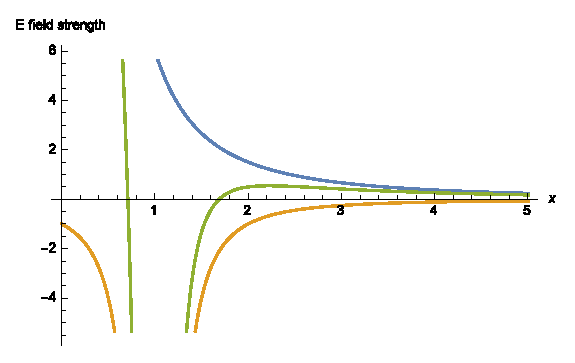
\includegraphics[width=.75\columnwidth]{1a_plot.eps}%
\caption{Plot of the electric field generated by the positive charge (blue), negative charge (orange) and sum of the two (green) - I have assumed d = 1 meter}%
\label{fig:1a_plot}%
\end{figure}


Okay, so now that we have solved for the two positions, let's see if we can provide some intuition about why there are two positions where $\vec{E} = 0$ and not just one. Below, in figure \ref{fig:1a_plot}, I show you the $\hat{x}$ component of the E-fields generated by each point charge individually from $ x = 0 \rightarrow 5d$ and their sum (green). Note that the $\hat{x}$ component of the E-field generated by the negative charge is \textbf{always reported as negative, even when $x$ is between $0$ and $d$ - i.e. between the two charges}. We know that when $x$ is between $0$ and $d$ we are between the two point charges. Between the two point charges the electric field due to the negative charge should point in the positive $\hat{x}$ direction.

So, what we have doesn't make any sense! The electric field from the negative charge should point to the right in between the two charges. The component of the electric field due to the negative charge should be positive between 0 and d and change sign abruptly at d such that it's negative for all $x >d$. It should look like figure \ref{fig:1a_neg_plot}.


How come? Well, remember when you were told that $\vec{E}_{\text{point\,charge}} = k q\frac{\hat{x}}{x^2}$. Well, this is only partly true. This is only true if your charge is located at the origin. In this case, the negative charge is not located at the origin (only the positive charge is). When the charge that you're considering is not at the origin you must consider the electric field generated by a point charge as follows.

\begin{align}
\vec{E}_{point\,charge} &= \frac{k q \hat{\pmb{\scriptr}}}{|\pmb{\scriptr}|^2} \nonumber \\
												&= \frac{k q \hat{\pmb{\scriptr}}}{|\pmb{\scriptr}|^2}\frac{|\vec{\pmb{\scriptr}}|}{|\vec{\pmb{\scriptr}}|} \nonumber \\
												&= \frac{k q \vec{\pmb{\scriptr}}}{|\pmb{\scriptr}|^3} \nonumber \\
												&=  \frac{k q ( \vec{R} - \vec{r} )}{|\vec{R}-\vec{r}|^3} \nonumber
\end{align}

\begin{figure}%
\centering
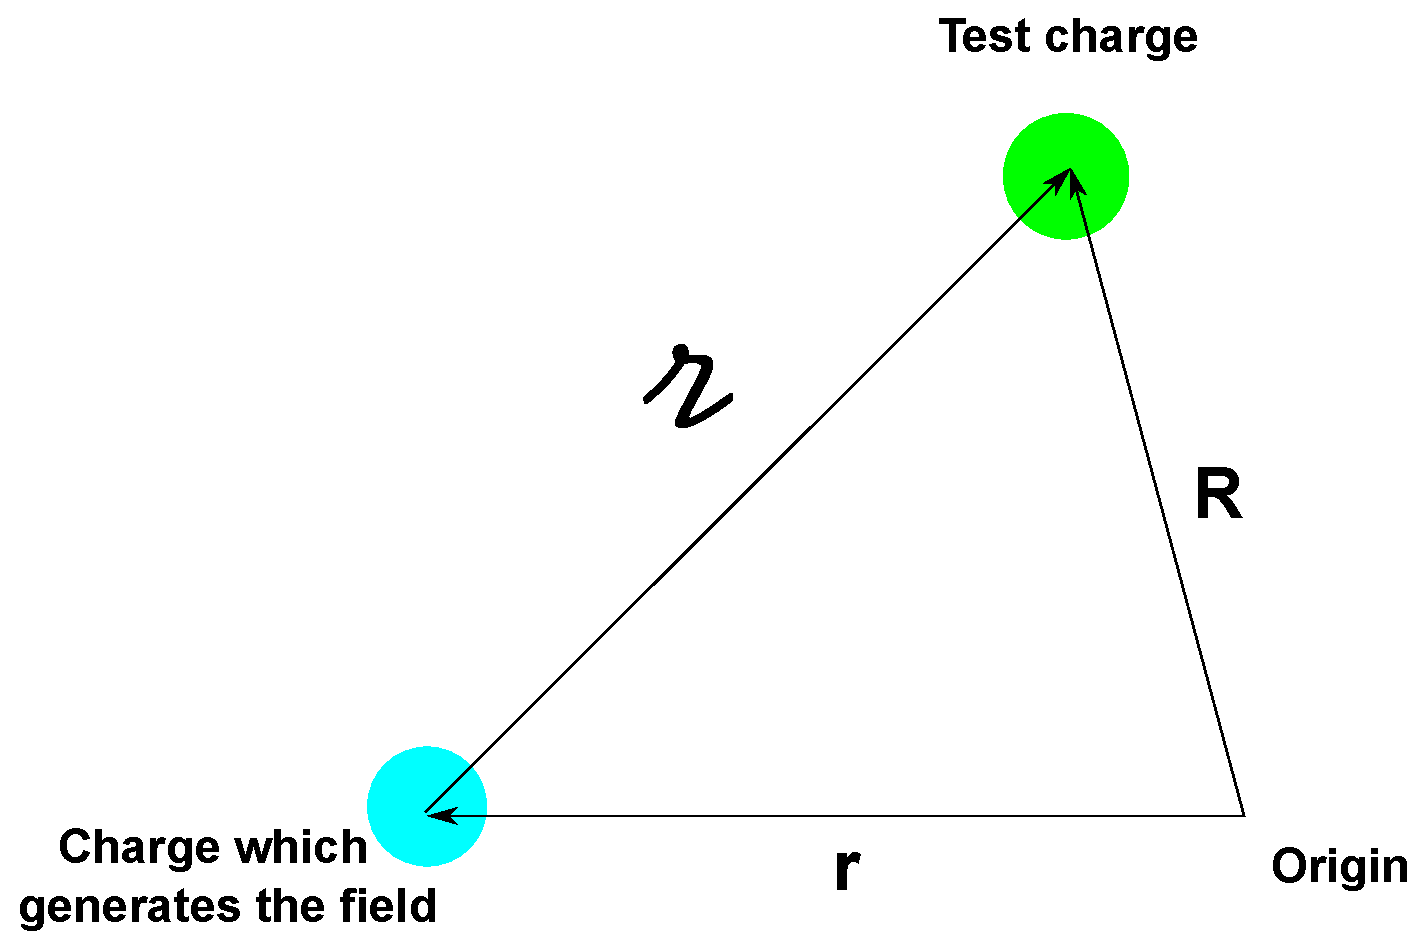
\includegraphics[width=.5\columnwidth]{1a_vec.eps}%
\caption{Pictorial representation of the three vectors involved in describing the electric field at a point in space due to a point charge}%
\label{fig:1a_vec}%
\end{figure}

You can refer to figure \ref{fig:1a_vec} for a pictorial representation of these vectors.

$\vec{r}$ is the vector that points from the origin to the charge that's generating the field we are interested in. In this problem, this charge is -q and is located at $d \hat{x}$.

$\vec{R}$ is the vector that points from the origin to us where the electric field needs to be calculated (in this problem, this is the position $x$ along the x axis: $\vec{R} = x\hat{x}$).

$\vec{\pmb{\scriptr}}$ is the vector that points from the charge (which is not at the origin) to us (the place where we want to calculate the electric field). It can be seen from figure \ref{fig:1a_vec} that $\vec{\pmb{\scriptr}} = \vec{R}-\vec{r}$. Thus, $\vec{\pmb{\scriptr}} = x\hat{x}-d\hat{x} = (x-d)\hat{x}$.



\begin{figure}%
\centering
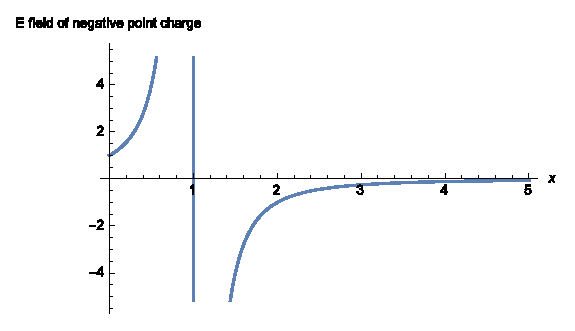
\includegraphics[width=.65\columnwidth]{1a_neg_plot.eps}%
\caption{Plot of the proper electric field generated by the negative charge for $5d>x>0$ - I have assumed d = 1 meter}%
\label{fig:1a_neg_plot}%
\end{figure}

So, $\vec{E}_{-q} = \frac{k (-q) (x-d)\hat{x}}{|x-d|^3} = \frac{k q (x-d)(-\hat{x})}{|x-d|^3} $. Note that this expression, a better expression for the electric field (it's more general), changes sign when x gets larger or smaller than d. This is exactly what we want. When $x < d$ (when we are to the left of the negative charge) the component of the electric field due to the negative charge should point in the positive $\hat{x}$ direction. When $x>d$ (when we are to the right of the negative charge) the component of the electric field due to the negative charge should point in the negative $\hat{x}$ direction. You can see that the expression just given does exactly that. I have plotted this electric field component in figure \ref{fig:1a_neg_plot}.

Note, that the expression I just gave you, which is more general, is the same as the prior expression used to find the solution for $x>d$. Based on a simple examination of the electric field behavior in between both charges we already know the solution has to be located where $x>d$. Thus, $ x \approx 1.69d$ is the solution to our problem.


\end{homeworkSection}
\begin{homeworkSection}{Problem 1b}

Another way that you could have read the problem statement is as follows.

Interpreted problem statement: \textbf{You are given two point charges, one positive and one negative. These two charges are separated by distance ``d''. The negative charge is} 6 times larger than the positive charge. \textbf{Where would you place a third charge so that the net electrostatic force on it is zero. Give answer in terms of ``d'' as measured from the positive charge.}

\begin{figure}%
\centering
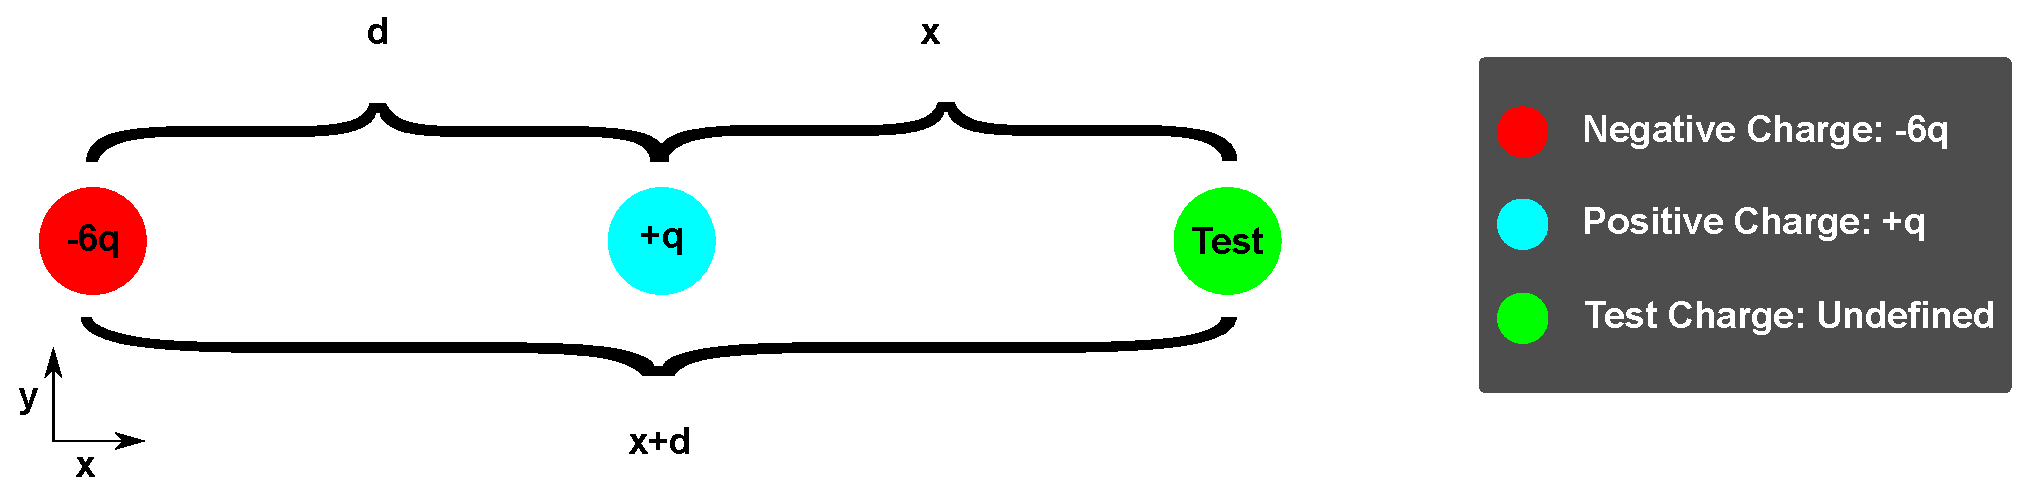
\includegraphics[width=\columnwidth]{1b.eps}%
\caption{Schematic for problem 1b. The key that describes the charges is redundant}%
\label{fig:1b.eps}%
\end{figure}

The problem is very similar as before, except for, now, instead of the larger charge being the positive charge, now, it is the negative charge. See figure \ref{fig:1b.eps} for a diagram. To make this solution simple for me to give you, without a bunch of math, I am going to appeal to my solution for 1a (please read that if you have not already). 

Notice that in this problem, no matter which charge has a larger magnitude, between either the positive or negative charge, the position where the electric field is zero is going to be the same. Namely, if the larger charge is positive (+6q), like it was in problem 1a, then the solution will be that the electric field is zero a distance of \textasciitilde1.69d from the positive charge and \textasciitilde.69d from the negative charge. If the larger charge is negative (-6q), like it is in problem 1b, then the solution will be \textasciitilde1.69d from the negative charge and \textasciitilde.69d from the positive charge: The same distance from the larger of the two charges.

I encourage you to prove this to yourself by writing the equations that prove this. I'm not saying that the electric field \textbf{everywhere in space} is the same for both the configuration in problem 1b and in problem 1a. On the contrary: The electric field points in the positive $\hat{x}$ direction between the two charges in problem 1a and in the negative $\hat{x}$ direction between the two charges is problem 1b. It is only the location of zero electric field that is the same in both problems.

Now, that we know this, we know exactly where the position of zero electric field is for this problem. It is \textasciitilde1.69d from the negative charge (since it has a larger magnitude). This means that the electric field is zero a distance of  \textasciitilde 1.69d - d = \textasciitilde.69d away from the positive charge since the positive charge is d away from the negative charge (see figure \ref{fig:1b.eps} for a picture that might help explain this).
\end{homeworkSection}

\section{Conclusion}
Okay, I'm done explaining quiz problem \#1. If you have any questions then you are more than free to ask me in person. Otherwise, I will see you on Friday for our next tutorial. Thank you very much for reading this.
\end{homeworkProblem}